\documentclass[a4paper, 12pt]{article}

\usepackage[utf8]{inputenc}%encodage des caractères
\usepackage[T1]{fontenc}%encodage de la police
\usepackage[french]{babel}%langue française
\usepackage{hyperref}
\usepackage{dirtree}
\usepackage{listings}
\usepackage{color}
\usepackage{graphicx} %affichage des images
\usepackage{float}
\usepackage[top=3cm,bottom=3cm,left=3cm,right=3cm]{geometry}

\lstset{
  tabsize=2,
  breaklines=true
}

\newcommand{\inline}[1]{\texttt{#1}}

\title{Rapport de TPA \\ Programmation chimique}
\author{Oumaima Chammakhi \and Guillaume Chauveau \and Amadou Keita \and Chloé Le Gentil}
\date{5 avril 2019}

\begin{document}
\begin{figure}
  
\includegraphics{img/logo.png}
\end{figure}
\maketitle
\thispagestyle{empty}
\setcounter{page}{0}

\pagebreak
\tableofcontents
\pagebreak

\section{Introduction}
Afin de bien maîtriser la programmation orientée objet, plus précisément le langage Java, une sélection de projet à réaliser nous a été proposée. Parmi les sujets, la programmation chimique a retenu notre attention.

La programmation chimique est un modèle de programmation qui s’inspire, comme son nom l’indique, de la chimie, mais aussi de la biologie. Ce modèle, appelé P système, imite les réactions entre des éléments chimiques à l’intérieur de cellules (ou membranes). Ces éléments réagissent entre eux selon des règles préétablies. L’ensemble des cellules, des règles et des éléments de départ décrit un programme chimique. Le déroulement d’un programme chimique, aussi appelé solution, est non-déterministe car les éléments réagissent entre eux aléatoirement (pour simuler une réaction chimique réelle).

L’objectif de ce projet est de créer un interpréteur de programmes chimiques, ainsi qu’un parseur qui permet à l’utilisateur de décrire son programme dans un fichier à l’aide d’un langage simple. L’interpréteur doit être capable d’exécuter un sous-programme en parallèle, représenté par une sous-cellule. Les différents programmes doivent pouvoir échanger des éléments verticalement, c’est-à-dire d’un programme à l’un de ses sous-programmes et vice-versa.

\begin{figure}[!ht]
  \centering
  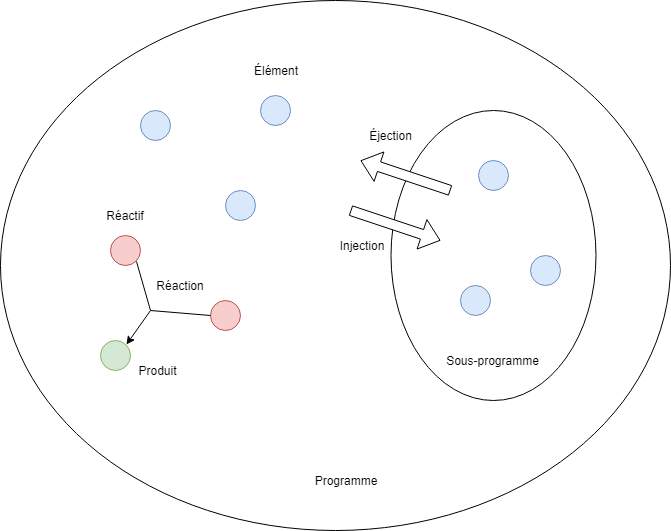
\includegraphics[scale=0.5]{./img/Programme.png}
  \caption{Schéma représentant un programme avec ses éléments et ses sous-programmes}
\end{figure}

Nous avons choisi de nommer notre projet P6 (pour P système). En plus des fonctionnalités demandées par la consigne, nous avons découpé le projet en différents modules que nous détaillerons dans la partie suivante, dans l’objectif de permettre à l’utilisateur d’étendre les capacités de l’interpréteur facilement.

\section{Structure du projet}
\subsection{Architecture}
P6 est constitué de trois composants principaux :
\begin{itemize}
  \item Le noyau
  \item Les bibliothèques
  \item Le parseur
\end{itemize}
Ces composants sont ensuite utilisés par des applications intégrées à P6, ou directement par l’utilisateur dans un programme Java.

\subsubsection{Le noyau}
Le noyau est le composant principal. Il décrit de manière abstraite les éléments chimiques et les règles de réaction. Il décrit aussi les cellules, avec leurs éléments, règles et sous-cellules. Enfin, le noyau est responsable de l’exécution d’un programme, grâce à un (ou plusieurs) réacteur.

\begin{figure}[!ht]
  \centering
  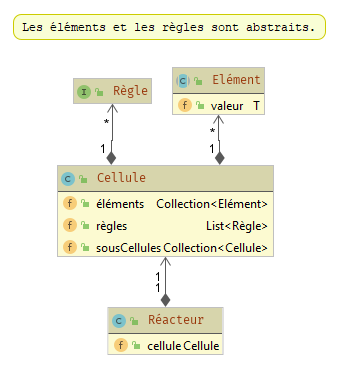
\includegraphics[scale=0.8]{./img/Structure_noyau.png}
  \caption{Illustration simplifiée des classes du noyau}
\end{figure}

\subsubsection{Bibliothèques}
Les bibliothèques implémentent les concepts abstraits décrits dans le noyau, c’est-à-dire les éléments et les règles. Les éléments sont typés, et les règles qui s’appliquent dépendent généralement du type des éléments. Des règles qui ne dépendent pas d’un type en particulier sont aussi proposées. Le but principal du projet n’est pas de proposer des bibliothèques très complètes pour plusieurs types d’éléments différents, mais plutôt de permettre à l’utilisateur de créer ses propres implémentations. Les différentes bibliothèques sont rassemblées en un point d’accès centralisé, le registre des bibliothèques.

\begin{figure}[!ht]
  \centering
  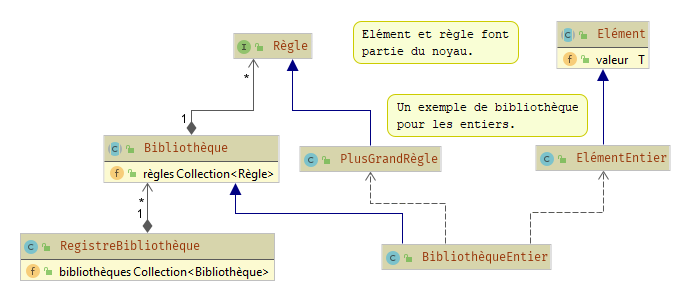
\includegraphics[scale=0.7]{./img/Structure_bibliotheque.png}
  \caption{Illustration simplifiée de la gestion des bibliothèques}
\end{figure}

\subsubsection{Parseur}
Ce module propose un outil permettant de créer une solution (un programme) complète en utilisant un langage spécialisé, afin de s’affranchir de l’API Java du noyau. Les règles de réactions sont simplement nommées, leur implémentation devant être définie dans le registre des bibliothèques. Il n’est pas possible de décrire directement le comportement de celles-ci dans le code source parsé. La syntaxe, inspirée du \href{https://json.org/}{JSON}, permet d’indiquer un nom, les règles, éléments de départ ainsi que les sous-cellules associés à chaque cellule. Un fichier de programme P6 consiste alors à décrire la cellule racine (le programme principal), puis, le cas échéant, ses sous-cellules.

\subsubsection{Applications}
P6 propose actuellement une application en ligne de commande permettant de lancer un programme contenu dans un fichier, mais aussi un utilitaire ajoutant une couche d’abstraction à l’API du noyau et du registre pour créer une solution dans un programme Java.

\subsubsection{Récapitulatif}
Pour résumer, P6 est constitué de différent module qui dépendent les uns des autres. Ils seront détaillés dans leur partie respective par la suite, mais nous allons tout d’abord nous intéresser à la gestion concrète du projet.

\begin{figure}[!ht]
  \centering
  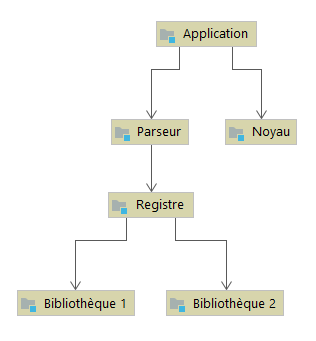
\includegraphics[scale=0.8]{./img/Structure.png}
  \caption{Illustration simplifiée des relations entre les modules du projet}
\end{figure}

\subsection{Utilisation de Gradle pour la gestion du projet}
Utiliser directement le compilateur Java était impensable pour un projet de cette taille, nous nous sommes donc penchez vers Gradle pour automatiser certaines tâches. Gradle est l’automate de production officiel pour la création d’applications Android et est décrit par Wikipédia comme alliant les atouts de Maven et Ant, ses principaux compétiteurs. Avoir de l’expérience avec cet outil nous a semblé judicieux puisque nous travaillerons sur des applications mobiles en L3.
Une fonctionnalité clé de Gradle que nous utilisons est la possibilité de séparer le code en sous-projet. Ainsi, chaque module de P6 est un sous-projet Gradle, ce qui permet de les cloisonner plus efficacement, et de gérer plus élégamment les dépendances entre les modules. L’exemple le plus flagrant est la dépendance d’une application avec les bibliothèques lors de l’exécution, mais pas à la compilation. Nous aurons l’occasion d’expliquer cette différence dans la partie dédiée aux bibliothèques.
\pagebreak
\subsection{Arborescence des dossiers}
\dirtree{%
  .1 .
  .2 cli/\DTcomment{Dossier de l'application en ligne de commande}.
  .3 src/main/java/com/p6/cli/\DTcomment{Sources de l'application}.
  .2 core/\DTcomment{Module du noyau}.
  .3 src/main/java/com/p6/core/\DTcomment{Sources du noyau}.
  .4 genesis/\DTcomment{Package pour la génération d'éléments}.
  .4 reaction/\DTcomment{Représentation des règles}.
  .4 reactor/\DTcomment{Exécution d'un programme}.
  .4 solution/\DTcomment{Représentation d'une cellule}.
  .2 dist/\DTcomment{Dossier de distribution}.
  .3 demos/\DTcomment{Programmes P6 et code Java de démonstration}.
  .3 scripts/\DTcomment{Scripts pour la distribution et les démonstrations}.
  .2 expression/\DTcomment{Dossier du rapport et de la présentation}.
  .2 gradle/\DTcomment{Dossier de gestion Gradle}.
  .2 lib/\DTcomment{Module de gestion des bibliothèques}.
  .3 common/\DTcomment{Bibliothèque P6 non spécifique à un type d'élément}.
  .4 src/main/java/com/p6/lib/common/\DTcomment{Dossier source}.
  .5 reaction/\DTcomment{Règles générales}.
  .5 solution/\DTcomment{Types d'élément abstraits}.
  .3 integers/\DTcomment{Bibliothèque P6  pour les nombres entiers}.
  .4 src/main/java/com/p6/lib/integers/.
  .5 genesis/\DTcomment{Génération d'éléments à nombre entier}.
  .5 reaction/\DTcomment{Règles sur les nombres entiers}.
  .5 solution/\DTcomment{Représentation des éléments à nombre entier}.
  .3 src/main/java/com/p6/lib/\DTcomment{Sources de la gestion}.
  .2 parser/\DTcomment{Module du parseur}.
  .3 src/main/java/com/p6/parser/\DTcomment{Sources du parseur}.
  .2 utils/\DTcomment{Module contenant des classes utilitaires}.
}


Nous allons à présent détailler le fonctionnement ainsi que certains aspects techniques des modules.

\section{Le noyau}
Le noyau remplit trois rôles primordiaux dans l’utilisation de P6.

\subsection{Représentation d'une solution}
Son premier rôle est de proposer des classes représentant le programme. La classe \inline{com.p6.core.solution.Cell} représente une cellule. Elle est constituée d’une liste de règles de réaction, une liste d’éléments ainsi qu’une liste de sous-cellules. Elle a aussi une référence vers sa cellule parente, dans le cas où elle est un sous-programme. Différentes méthodes permettent de vérifier son état ou de le modifier. On peut lui ajouter des éléments ou règles, ajouter ou supprimer des sous-cellules mais aussi effectuer des opérations entre les cellules comme l’injection d’éléments dans une sous-cellule spécifique, l’éjection d’éléments dans la cellule parente et enfin déclencher la  dissolution de la cellule. Une cellule qui se dissout éjecte tous ses éléments dans son parent, ainsi que ses sous-cellules. La cellule dissoute est ensuite retirée de la liste des enfants de la cellule parente. Cette classe propose aussi une méthode qui permet de choisir un élément qu’elle contient au hasard. Cet élément est retiré de la cellule. La classe \inline{com.p6.core.solution.Element<T>} sert de base aux implémentations d’éléments qui lui fixe son type. Elle est porteuse d’une valeur qui est utilisée lors des réactions.

\begin{figure}[!ht]
  \centering
  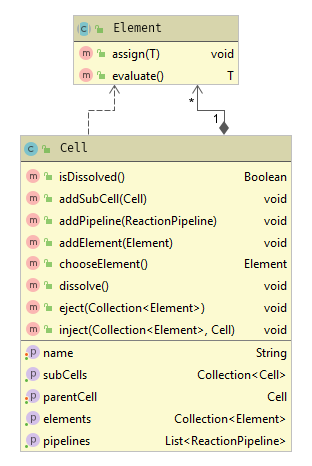
\includegraphics[scale=0.8]{./img/Core_solution.png}
  \caption{Graphique UML des classes représentant un programme}
\end{figure}

\subsection{Représentation des règles}
Les règles de réaction sont appliquées lors de l’exécution sur deux éléments sélectionnés aléatoirement dans la cellule. Elles aboutissent généralement à la création d’éléments dits produits, en consommant les éléments de départ (les réactifs). Il est possible que la réaction ne puisse avoir lieu, dans le cas où des conditions spécifiées par la règle ne sont pas remplies. Afin de garantir une grande flexibilité lors de l’écriture des règles par l’utilisateur, le noyau les représente sous la forme d’un processus en étapes appelé pipeline de réaction. Chaque étape du pipeline reçoit des éléments en entrée et doit retourner des éléments de sortie ou indiquer que les réactifs ne respectent pas les conditions nécessaires. Dans le cas où l’étape se déroule normalement, son résultat est passé à l’étape suivante et ainsi de suite jusqu’à la fin du pipeline. Les produits sont alors ajoutés à la cellule.

\begin{figure}[!ht]
  \centering
  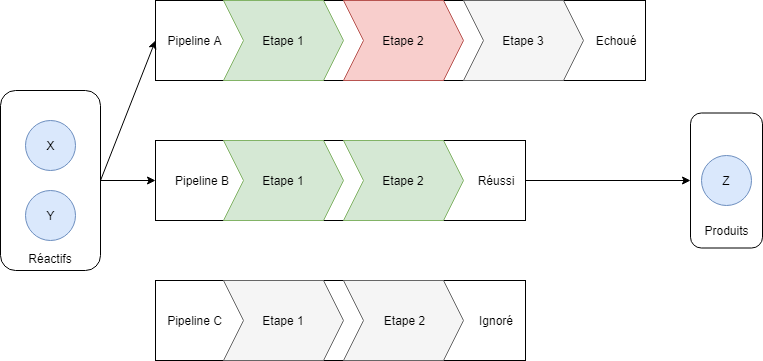
\includegraphics[scale=0.5]{./img/Pipeline.png}
  \caption{Exemple de déroulement d'une réaction dans une cellule avec trois pipelines}
\end{figure}

Un pipeline (\inline{com.p6.core.reaction.ReactionPipeline}) est donc constitué d’une liste d’étapes de pipeline (\inline{com.p6.core.reaction.ReactionPipelineStep}). Ce sont ces étapes qui sont implémentées par les bibliothèques. Elles doivent notamment vérifier le type des éléments en entrée afin de déterminer s’ils peuvent réagir ensemble. S’ils ne sont pas compatibles, on dit que le pipeline a échoué. L’exécuteur de programme, le réacteur, va alors essayer le pipeline suivant de la cellule.

\begin{figure}[!ht]
  \centering
  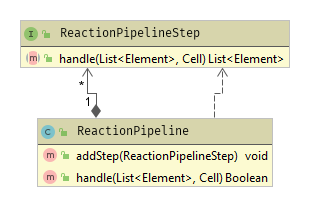
\includegraphics[scale=0.8]{./img/Core_reaction.png}
  \caption{Graphique UML des classes représentant une règle de réaction}
\end{figure}

\subsection{Exécution d'un programme}
Le troisième rôle du noyau est l’exécution complète d’un programme. Deux types d’objet entrent en jeu : les réacteurs (\inline{com.p6.core.reactor.Reactor}) et le coordinateur de réacteur (\inline{com.p6.core.reactor.ReactorCoordinator}).
Il y a un réacteur assigné à chaque cellule, sous-cellule. Il exécute le programme de la cellule en sélectionnant deux éléments au hasard et en tentant de les faire passer dans les pipelines de réaction. Dès que le pipeline réussi, ses produits sont ajoutés à la cellule. Si tous les pipelines ont échoué, il n’y a pas de réaction, les réactifs sont remis dans la cellule. Cette non-réaction est enregistrée par un compteur de stabilité, qui va permettre de déterminer quand arrêter le réacteur. Lorsque que la cellule atteint un seuil prédéfini de stabilité ou que le réacteur est a effectué un certain nombre de réaction (appelé nombre d’itération), le programme de la cellule est terminé.

Les réacteurs sont créés et lancés en parallèle par le coordinateur. Cet objet prend la cellule racine ainsi que le nombre d’itération maximum et le seuil (la cible) de stabilité et parcourt l’arbre formé par les cellules pour assigner un nouveau réacteur à chaque cellule. On peut alors démarrer l’exécution du programme complet, où chaque réacteur travaille dans son propre processus léger (thread). Cette méthode d’exécution ajoute une autre dimension aléatoire au programme chimique, puisque les réacteurs ne travaillent réellement que lorsque le planificateur du système d’exploitation leur donne du temps.

\begin{figure}[!ht]
  \centering
  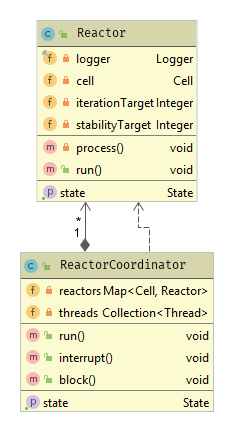
\includegraphics[scale=0.8]{./img/Core_reactor.png}
  \caption{Graphique UML des classes d'exécution de programme}
\end{figure}

\section{Les bibliothèques}
Les bibliothèques contiennent les classes concrètes pour les éléments ainsi que les étapes de pipeline de réaction. Elles implémentent aussi des générateurs d’éléments (\inline{com.p6.core.genesis.ElementGenerator}), utilisés lors de la création des cellules pour ajouter les éléments de l’état initial. Le registre des bibliothèques va conserver une liste de toutes les étapes ainsi que tous les générateurs définis par les bibliothèques, afin de pouvoir y accéder facilement à l’aide d’un nom unique. Ces deux types d’objet peuvent avoir des arguments. Un intermédiaire chargé de créer l’instance à partir d’un tableau d’arguments est donc introduit avec l’interface \inline{com.p6.lib.InitArgsParser<T>}. Cette interface fonctionnelle possède une méthode qui retourne la nouvelle instance de \inline{T}. La classe principale d’une bibliothèque (\inline{com.p6.lib.Library}) possède deux méthodes retournant des associations nom / interface d’initialisation, pour les générateurs d’éléments et les étapes de pipeline de réaction qu’elle fournit.

\begin{figure}[!ht]
  \centering
  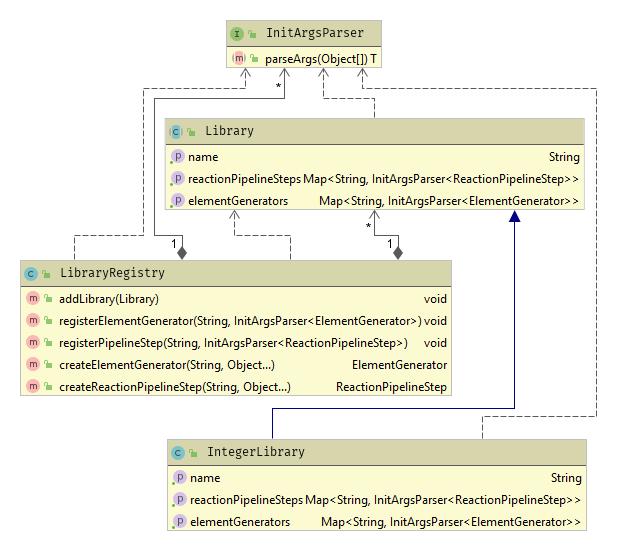
\includegraphics[scale=0.8]{./img/Library.png}
  \caption{Organisation des bibliothèque avec un exemple de bibliothèque pour les entiers}
\end{figure}

La bibliothèque peut enfin être ajoutée au registre. Cela peut être fait avec l’une de ses méthodes, mais les \href{https://docs.oracle.com/javase/tutorial/ext/basics/spi.html}{services Java} offrent une alternative plus intéressante. Le registre charge automatiquement tout service implémentant la classe \inline{Library}. L’utilisateur peut ainsi utiliser sa bibliothèque sans recompiler son application (comme le lanceur de programme fourni avec P6). Il suffit que la bibliothèque soit accessible dans le chemin de classes Java et que le fichier correspondant à la classe des bibliothèques, \inline{com.p6.lib.Library}, soit correctement rempli dans le dossier \inline{META-INF/services} (le dossier de démonstration du projet donne un exemple).

\section{Le parseur}
Le parseur permet la création d’un programme P6 depuis une chaîne de caractères grâce à une syntaxe. Le processus se déroule en deux étapes : le parseur commence par analyser la chaîne en entrée (appelée source) pour en extraire sa structure, puis créer le programme correspondant à la structure.

\subsection{Analyse de la forme}
Dans cette première étape, il n’est pas encore question de cellule, pipeline ou générateur. L’objectif est de créer une structure de données correspondant à la source. La syntaxe employée est proche du JSON, on retrouve notamment trois types de structures :
\begin{itemize}
  \item Les chaînes de caractères
  \item Les listes
  \item Les associations clé / valeur
\end{itemize}
Les listes sont délimitées par des crochets ouvrants et fermants. Il est important de noter que chaque structure doit débuter sur sa propre ligne. Une liste de chaînes de caractères s’écrit alors :
\begin{lstlisting}
[
	Ma chaine de caracteres
]
\end{lstlisting}
Il en va de même pour les associations, délimitées par des accolades :
\begin{lstlisting}
{
  Cle : valeur
}
\end{lstlisting}
Il est possible de faire des listes de structures, comme des listes d’associations, mais aussi des associations avec des structures. Les clés d’une association sont toujours des chaînes de caractères. Les objets Java correspondants à ces structures sont :
\begin{itemize}
  \item \inline{String}
  \item \inline{List<Object>}
  \item \inline{Map<String, Object>}
\end{itemize}
La gestion des erreurs est basique mais permet la détection de structure non terminées, comme dans le cas où un crochet serait manquant pour une liste. Les structures se terminant avant même d’avoir commencé sont aussi repérées.
C’est la classe \inline{com.p6.parser.StructureParser} qui est chargée de cette étape. La structure Java correspondant à la source est ensuite analysée par \inline{com.p6.parser.CellParser} afin de créer le programme.

\pagebreak
\subsection{Création du programme}
Un programme (ou sous-programme) est représenté par une cellule. Le parseur à besoin d’un nom, d’une liste de pipelines de réaction ainsi qu’une liste de générateurs d’élément pour créer une cellule. Une liste de sous-cellule peut être ajoutée. La syntaxe correspondante ressemble à :
\begin{lstlisting}
# Cette ligne est un commentaire grace au diese.
{
  name: Ma cellule # Le nom de la cellule.
  elements : [ # La liste des generateurs.
    monGenerateur
  ]
  rules: [ # La liste des pipelines (regles).
    x, y : etape1 : etape2($y)
  ]
  subCells: [ # Optionnellement, la liste des sous-cellules.
    { # Debut de la sous-cellule.

    }
  ]
}
\end{lstlisting}

Le parseur commence par vérifier que la structure correspond au schéma prévu, puis lance récursivement la création des sous-cellules pour permettre leur utilisation par la suite. Il enregistre ensuite directement dans la nouvelle cellule les informations qui ne nécessitent pas de traitement supplémentaire (comme le nom).
Les générateurs et les pipelines requièrent une étape en plus. Ils sont décrits par une liste d’instructions, une chaîne de caractères de la forme \lstinline{(preambule :) instruction1 : instruction2(argument1, $reference1) ...}. Une instruction correspond à une étape de pipeline ou à un générateur. La liste d’instructions d’un générateur ne doit donc contenir qu’une seule instruction. Le nom de l’instruction (la partie avant les arguments) sert à retrouver l’interface d’initialisation correspondant dans le registre des bibliothèques. Les arguments seront passés sous forme de chaîne de caractères, mais ceux dont le premier caractère est un dollar seront remplacés par une référence. Les références sont définies par une association chaine de caractères / objet dans le parseur. Cette association contient des informations relatives au contexte, comme les références des sous-cellules. Une référence avec le nom d’une sous-cellule sera donc remplacée par la sous-cellule elle-même.
Le préambule optionnel est utilisé lors des descriptions de pipelines pour référencer le premier élément (celui de gauche) du pipeline et le deuxième (de droite). Les pipelines ont donc la forme \lstinline{elementGauche, elementDroit : etape1($elementGauche, argument1) : etape2($sousCellule) : etape3}. Les références sur les éléments de gauche ou droite sont remplacées par la valeur correspondante dans l’énumération \inline{com.p6.core.solution.Element.Side}. Les étapes peuvent ensuite interpréter sa signification comme elles le souhaite. Par exemple, l’étape \inline{choose} définie par \inline{com.p6.lib.common.reaction.ChooseElement} ne va retourner que le premier élément du pipeline ou le deuxième, alors que \inline{sortInt} va trier les éléments entier du plus grand au plus petit si la référence en paramètre est à gauche, ou du plus petit au plus grand si elle est à droite.
Une fois les générateurs d’élément et les pipelines de réaction correctement initialisés et ajoutés, la cellule est prête à être exécutée.

\begin{figure}[!ht]
  \centering
  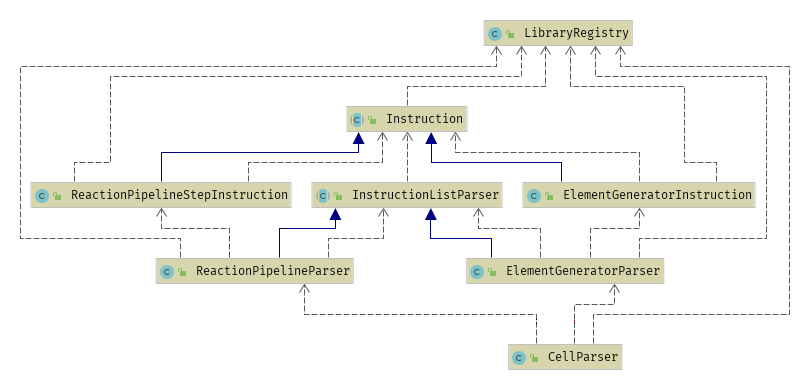
\includegraphics[scale=0.6]{./img/Parser.png}
  \caption{Structure interne du parseur}
\end{figure}

\section{Applications}
Les modules que nous avons présentés permettent de créer et exécuter séparément un programme P6, mais c’est le rôle des applications de coordonner leur utilisation.

\subsection{Le lanceur de programme en ligne de commande}
La seule application utilisable directement fournie par P6 est le lanceur de programme en ligne de commande, ou CLI. Cette application se présente sous la forme d’un exécutable (une archive JAR ou un script) auquel l’utilisateur doit passer en argument le chemin vers un fichier texte contenant le programme, la cible d’itération et la cible de stabilité. Le contenu final des cellules sera affiché dans la sortie standard (les messages de journal sont eux dans la sortie d’erreurs). Il est possible d’exporter l’état final des cellules dans un fichier avec les détails des types en utilisant le drapeau \inline{--output} suivi d’un chemin vers un fichier. Les résultats sont enregistrés sous la forme :

\begin{lstlisting}
Nom_de_la_cellule Classe_de_l-element Representation_de_la_valeur
.
.
Nom_de_la_sous_cellule ...
.
.
.
---
\end{lstlisting}

où \inline{---} indique la fin des sous-cellules (chaque cellule se termine par cette séquence). Ce fichier peut ensuite être utilisé pour des traitements supplémentaires.
CLI propose d’autre options comme la possibilité d’afficher les résultats des réactions lentement (avec le drapeau \inline{--verbose}) ou de n’afficher que les erreurs (avec \inline{--quiet}). Nous utilisons le framework \href{https://picocli.info/}{PicoCLI} pour simplifier le traitement des arguments. Toutes les options peuvent être affichées avec \inline{--help}.

\subsection{Utilisation de l'API pour créer et exécuter son programme}
L’utilisateur peut aussi utiliser P6 dans sa propre application Java en passant par l’interface de programmation d’application (API) des différents modules. Créer son programme avec l’API du noyau peut se montrer très verbeux, puisqu’il faut d’abord instancier de nombreuses classes avant de les assembler pour obtenir le programme complet. C’est pourquoi nous avons créé un utilitaire dans le module des bibliothèques (\inline{com.p6.lib}) nommé \inline{SolutionBuilder}. Chaque instance de cette classe va correspondre à une solution (un programme). La création de la solution commence par la cellule racine, que l’on initialise avec la méthode \inline{createCell()}. Cette méthode va retourner l’instance de la classe \inline{Cell} qui vient d’être créée, utile dans le cas de sous-cellules pour la configuration de certaines étapes de pipeline. On peut ensuite appeler la méthode \inline{addElement()}, pour ajouter un ou plusieurs éléments ou ceux générés par un générateur d’éléments. L’ajout de pipeline s’effectue d’une manière similaire à la création d’une cellule : on commence par l’initialiser avec \inline{createPipeline()}, puis on peut ajouter des étapes en appelant \inline{addStep()}. Lorsque la méthode \inline{createPipeline()} est rappelée, pour configurer un deuxième pipeline par exemple, le pipeline en cours de configuration est verrouillé et ajouté à la cellule. Pour ajouter des sous-cellules, il suffit d’utiliser une nouvelle fois la méthode \inline{createCell()}. Pour éviter d’ajouter une cellule enfant à la cellule courante mais plutôt lui créer une cellule soeur (qui a la même cellule parente), il faut d’abord sceller la cellule avec \inline{sealCell()}. La cellule ne pourra plus être modifiée et le pipeline en cours de création est ajouté. La cellule racine doit elle aussi être scellée avant de pouvoir récupérer la solution complète avec la méthode \inline{getSolution()}. La cellule retournée par cette dernière opération peut maintenant être exécutée par un coordinateur de réacteur normalement.

\begin{figure}[!ht]
  \centering
  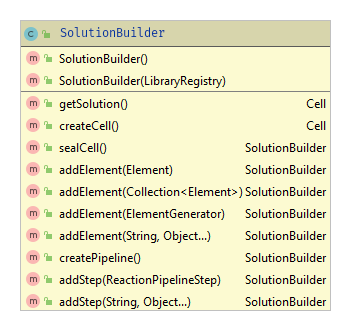
\includegraphics[scale=0.8]{./img/SolutionBuilder.png}
  \caption{Graphique UML de l'utilitaire}
\end{figure}

\subsection{Le prototype d'interface graphique}
Le prototype d’interface graphique avait pour but de modéliser graphiquement notre programme. Cependant, la modélisation d’un trop grand nombre d’éléments étant compliqué, nous avons décidé de simplifier la version graphique du programme P6 en le réduisant à un certain nombre d’élément.
Ainsi nous avons pu travailler sur l’interprétation graphique d’une réaction entre plusieurs éléments.
Par manque de temps, nous avons choisi de mettre le prototype d’interface graphique de côté, afin de nous focaliser sur les éléments nécessaires au bon fonctionnement de notre programme.

\section{Conclusion}
Notre projet répond aux objectifs fixés mais a encore une grande marge d’amélioration. Le réacteur du noyau doit être configuré par l’utilisateur pour pouvoir être utilisé. On pourrait imaginer un système qui estime les paramètres du réacteur grâce à un échantillon de la population des éléments de la cellule, dans le cas de programmes travaillant sur de grands volumes. Dans ce même cas, le traitement des éléments d’une même cellule pourrait être parallélisé. Nous avons exploré la possibilité d’utiliser les capacités de parallélisation des cartes graphiques comme suggéré lors de la présentation du sujet, mais leur utilisation aurait demandé d’importantes modifications au fonctionnement du noyau et des bibliothèques. Pour les applications, l’idée d’une interface graphique nous avait intéressé dès le début, mais la réalisation n’est restée qu’au prototypage. Enfin, nous avons pu utiliser notre projet pour exécuter des programmes simples sur des entiers, mais n’avons pas trouvé d’exemples plus complexes utilisant les fonctionnalités autour des sous-cellules.
La documentation sur la programmation chimique est plutôt restreinte, et les projets que nous avons trouvés semblent être plus expérimentaux que des solutions à un problème répandu, à l’inverse des nombreux outils d’apprentissage machine, par exemple. Ce sont souvent des projets universitaires liés à des recherches théoriques sur le sujet.

\end{document}
